\chapter{Resultados}
\label{chap:resultados}
Este capítulo irá mostrar os resultados da comparação dos sistemas criados, um que utiliza a persistência monoglota e outro que utiliza a persistência poliglota. O modelo de persistência poliglota tinha como alvo melhorar o desempenho da página \verb|feed|, mas sabemos que para isso a escrita do \textit{tweet} iria ser mais lenta. Pois, ao usuário publicar o \textit{tweet} é necessário atualizar o \textit{feed} de todos os seguidores desse usuário. Então iremos comparar o tempo de consulta do \textit{feed} de \textit{tweets} e o tempo de inserção de um \textit{tweet}.

O capítulo foi dividido em três seções: a \autoref{sec:resultFeed} que descreve como os testes foram realizados para medir tempo de consulta do \textit{feed} de \textit{tweets}, a \autoref{sec:resultInsertTweet} que descreve como foram feitos os testes para medir o tempo de inserção de um \textit{tweet} e a \autoref{sec:resultEval} irá analisar os resultados encontrados.

Para medir o tempo das operações utilizamos uma classe do próprio \textit{Ruby}, chamada \textit{Benchmark}\footnote{A documentação da classe Benchmark. \url{http://www.ruby-doc.org/stdlib-2.0/libdoc/benchmark/rdoc/Benchmark.html}}. Dessa classe utilizamos o método chamado \textit{measure} que mede o tempo de execução. Nesse tempo está incluído o tempo da operação no banco de dados e o tempo do carregamento dos valores para as variáveis do sistema.

Os testes foram realizados na máquina Asus, modelo N82J\footnote{A especificação se encontra sítio da Asus \url{http://www.asus.com/Notebooks_Ultrabooks/N82Jq/}} e o sistema operacional é Ubuntu 14.04 LTS.


\section{Resultados do tempo de consulta da \textit{feed} de \textit{tweets}}
\label{sec:resultFeed}

Para fazer um teste, no qual esses tempos medidos resultassem em uma diferença significativa criamos quatro bancos de dados no MongoDB. Esses bancos foram populados com cem usuários, porém a diferença entre os bancos foi a quantidade de \textit{tweets} de cada usuário. No primeiro banco de dados foram adicionados dez \textit{tweets} para cada usuário, totalizando mil \textit{tweets}. No segundo foram adicionados cem \textit{tweets} para cada usuário, totalizando dez mil \textit{tweets}, no terceiro banco foram adicionados mil \textit{tweets} para cada usuário totalizando cem mil \textit{tweets} e, por último, foram adicionados, no quarto banco de dados, dez mil \textit{tweets} para cada usuário, totalizando um milhão de \textit{tweets}.

Alteramos o primeiro usuário para seguir todos os outros noventa e nove usuários e executamos o método \verb|remake_feed| da classe \verb|User| para criar a chave no \ac{Redis}.

No modelo monoglota, medimos o tempo de execução da seguinte função:
\begin{lstlisting}
Tweet.in(user_id: user.following_ids).desc("created_at").
      paginate(:page => 1, :per_page => 100)
\end{lstlisting}

Essa função busca os cem \textit{tweets} mais recentes que o usuário atribuído ao objeto \textit{user} segue. Repetimos a execução dessa função cem vezes para cada banco de dados, que havíamos populado. Fizemos a média das cem repetições para cada banco e colocamos os resultados na \autoref{fig:time_feed_mono}.

\begin{figure}[H]
    \centering
    \caption{Tempo de consulta dos \textit{feeds} de \textit{tweets} com persistência monoglota}
    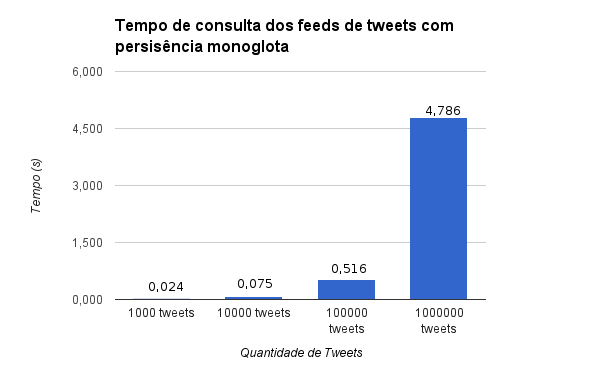
\includegraphics[width=0.8\textwidth]{./04-figuras/time_feed_mono.png}
    \label{fig:time_feed_mono}
\end{figure}


Podemos observar que o aumento da quantidade de \textit{tweets} foi quase diretamente proporcional ao tempo gasto.


No modelo poliglota, medimos o tempo de execução da seguinte função:
\begin{lstlisting}
	Tweet.feed_of user
\end{lstlisting}

Essa função busca no \ac{Redis} a chave do usuário \textit{user} que contém os cem \textit{tweets} mais recentes que esse usuário segue. Também medimos cem vezes para cada banco de dados, que havíamos populado. O tempo médio de leitura da chave foi em média menor que dois milésimos de segundos, independente da quantidade de \textit{tweets} cadastrados. Isso nos leva a uma melhora de desempenho grande, o sistema poliglota com um milhão de \textit{tweets} foi duas mil quinhentas e noventa e três vezes mais rápido que o sistema monoglota.

\section{Resultados do tempo de inserção de um \textit{tweet}}
\label{sec:resultInsertTweet}
Para realizar os testes de inserção de um \textit{tweet} criamos um banco de dados MongoDB com dez mil e um usuários, cada usuário com cem \textit{tweets}, totalizando mais de um milhão de \textit{tweets} e rodamos o método \verb|remake_feed| para polular o \ac{Redis}.

Alteramos a quantidade de seguidores do último usuário para cem, mil, e dez mil seguidores e, para cada conjunto de seguidores inserimos um \textit{tweet} cem vezes e medimos o tempo de cada inserção.

Para medir esse tempo de inserção em ambos os sistemas utilizamos a mesma função. A diferença da persistência poliglota é que foi criada uma função \textit{callback} que é executada após o \textit{tweet} ser criado. Essa função \textit{callback} realiza uma operação de leitura e outra de escrita no \ac{Redis} para cada seguidor. Ou seja, na implementação poliglota a cada \textit{tweet} inserido por um usuário, a chave de todos os seguidores desse usuário é refeita no \ac{Redis}.

Para a persistência monoglota, obtivemos os resultados rápidos e não variaram proporcionalmente com a quantidade de seguidores. Ou seja, a inserção no MongoDB obteve variações insignificantes. O tempo médio para cada conjunto de dados foi menor que um centésimo de segundo.
Já para a persistência poliglota, construímos um gráfico e uma tabela. O gráfico mostra o tempo total gasto para cada conjunto de seguidores e a tabela descreve o tempo gasto pelo \ac{Redis} e pelo MongoDB, conforme \autoref{fig:insert_poli} e \autoref{tab:percent_insert_tweet}, respectivamente.

\begin{figure}[H]
    \centering
    \caption{Tempo de inserção de um \textit{tweet} com persistência poliglota}
    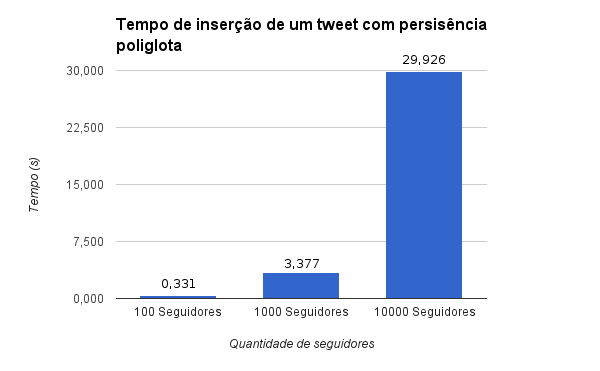
\includegraphics[width=0.8\textwidth]{./04-figuras/insert_poli.png}
    \label{fig:insert_poli}
\end{figure}

\begin{table}[H]
    \centering
    \caption[Comparação do tempo gasto pelos bancos MongoDB e Redis na inserção de um tweet]{Comparação do tempo gasto pelos bancos MongoDB e Redis na inserção de um \textit{tweet}.\label{tab:percent_insert_tweet}}
    \begin{tabular}{cccccc}
        \hline
            Qtd. de seguidores & Total (s) & MongoDB (s) & Redis (s) & \% MongoDB & \% Redis \\
        \hline
            100  & 0,314 & 0,010 & 0,331 & 3,06\% & 96,94\% \\
            1.000  & 3,388 & 0,011 & 3,377 & 0,32\% & 99,68\% \\
            10.000 & 29,937 & 0,011 & 29,926 & 0,04\% & 99,96\% \\
        \hline
    \end{tabular}
\end{table}



\section{Análise dos resultados}
\label{sec:resultEval}

Para a implementação monoglota tivemos piores resultados na consulta a \textit{feed} de \textit{tweets}. A média de tempo gasto aumentou significativamente quando a quantidade de \textit{tweets} no banco foram aumentados. Isso era esperado, pois para o banco encontrar os documentos procurados, foi necessário percorrer todos os \textit{tweets} e comparar com os parâmetros passados na consulta.
Já para a implementação poliglota, o tempo de execução para as diferentes quantidades de \textit{tweets} foram muito próximos, pois a consulta é apenas para buscar a chave, não havendo nenhuma outra comparação ou leitura a ser feita.
Podemos observar que tivemos uma melhora significativa, pois em nenhum momento a consulta a \textit{feed} de \textit{tweets} de um usuário foi mais rápida no sistema monoglota. Além disso, nos tempos medidos para um milhão de \textit{tweets} o sistema poliglota chegou a ser mais de duas mil e quinhentas vezes mais rápido.

Em relação aos resultados do tempo de inserção do \textit{tweet}, podemos observar que em nenhum instante a implementação poliglota foi mais rápida. Isso é devido ao tempo que foi gasto para atualizar as chaves. O aumento de seguidores foi proporcional ao aumento do tempo, ou seja, se aumentarmos em dez vezes os seguidores o tempo de atualização das chaves será, aproximadamente, dez vezes maior. A \autoref{tab:percent_insert_tweet} mostra que com o aumento de seguidores, o percentual de tempo gasto no MongoDB se torna menor e consequentemente o tempo gasto com o \ac{Redis} maior.
Isso porque, precisamos fazer uma leitura e uma escrita para cada chave ser atualizada, ou seja, operações no \ac{Redis}. Já para a implementação monoglota não houve diferença, pois a inserção de um \textit{tweet} não depende da quantidade de seguidores e está apenas vinculada ao MongoDB.

Não fizemos uma aplicação utilizando apenas o Redis, pois o tempo para desenvolver mais uma aplicação era curto. Sabemos que ao utilizar um banco desse gênero, iríamos ter ganhos ao acesso de informações diretas, como \textit{tweets} que o usuário logado publicou. Porém, qualquer consulta que precissasse verificar dados de algum valor da chave iria ter um pior desempenho. Por exemplo, ao pequisar \textit{tweets} que contém a palavra "josé", seria necssário percorrer e carregar para aplicação todos esses valores e fazer a comparação. Isso não acontece nos outros bancos, pois esses têm suporte para consulta.


